\chapter{Results and discussion}

The content of this chapter would be reported as the analysis 
procedure from step one to the end. The first part is the data 
correction process, count maps from the raw count as well as 
exposure map from the parallel computation, the spectrum and 
inversive fitting from heuristic optimization.

\section{Limb's angle correction}
Theoretically, the peak profile of the $\theta_\text{NADIR}$ would be
the same when time passes by.
From the observations, the nadir angle change through time 
evolving since the spacecraft altitude is gradually getting lower
in each year which will affect the LAT point of view when it sees 
the Earth.

\begin{figure}[h!]
    \centering
    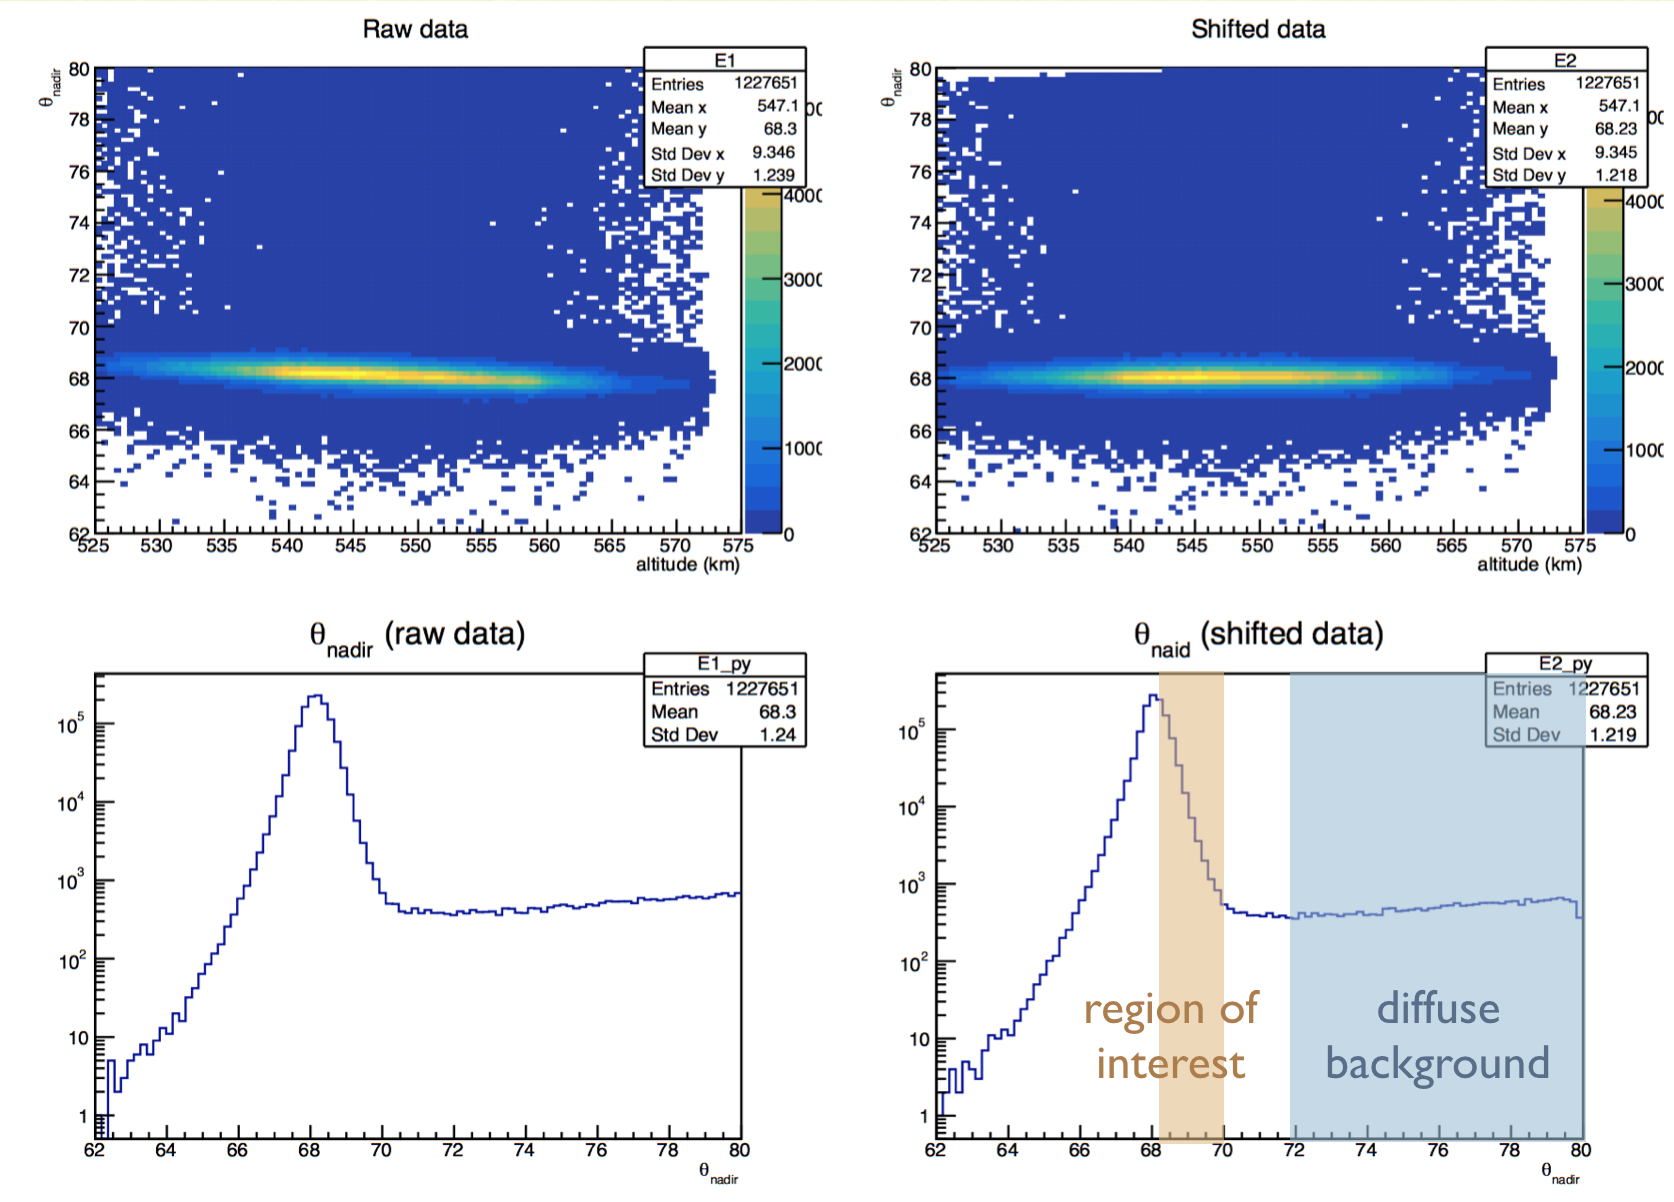
\includegraphics[width=0.8\textwidth]{content/result_and_discussion/figures/LATShifted.png}
    \caption{
        Distribution of nadir angle before and after altitude correction.
        (top) Heatmaps represents the photon density in axis
        of $\theta_\text{NADIR}$ versus altitude in kilometers.
        The left one came from raw data and the right one was
        converted by altitude shifting calculation.
        (bottom) The projected histograms from the above heatmaps
        in the axis of $\theta_\text{NADIR}$ where all photon
        from various altitudes was accumulated into the bin value.
    }
    \label{fig:lat_nadir_shifted}
\end{figure}


The top-left of Figure \ref{fig:lat_nadir_shifted} demonstrates how 
much spacecraft orbiting altitude correlate to the $\theta_\text{NADIR}$
by a 2D heatmap plot of photon intensity. The bottom-left histogram
came from the projection of the previous raw count 2-D histogram which 
has a peak around 68\textdegree. Both bottom and top right histograms
was constructed from the same logic but there is one different 
variable. The shifted nadir angle has been calculated to reduce the 
effect from the spacecraft and the region of interest has been highlighed 
as orange for calculating as the limb spectrum and the blue zone is 
a diffusive background to be used in the background subtraction.

The brightness of Earth's limb is much brighter than the 
diffusive background on the map. The region of interest and 
the background intensity has a huge difference in approximately
an order of magnitude.


\section{$\gamma$-ray spectrum measurement}

According to the definition from Equation \ref{eq:def_flux}, 
the first step is the construction of the count map of the Earth's 
centered coordinates. To illustrate how the outcome looks like,
we selected photon data from a single week due to the raw data
of photon from \textit{Fermi} was published once a week as one file.
A week of the accumulated photons is plotted in
the Figure \ref{fig:sample_photon_dist} to visualize 
the raw count of the sample data on the count map.

\begin{figure}[h!]
    \centering
        \subfloat[
            Heatmap of photon density in nadir angle where the 
            radius direction is the azimutal nadir
            angle ($\theta_\text{NADIR}$).
        ]{
            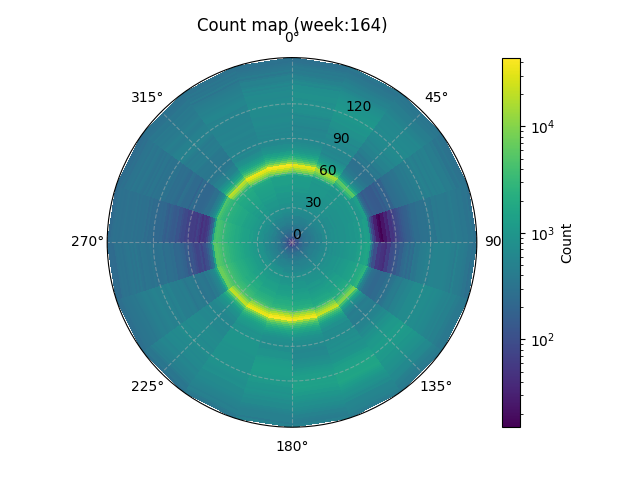
\includegraphics[width=0.47\textwidth]{content/result_and_discussion/figures/cntmap_polar.png}
        }
        \hfill
         \subfloat[
            A projected histogram from the heatmap.
            The x-axis is $\phi_\text{NADIR}$ from 0\textdegree
            to 360\textdegree.
        ]{
            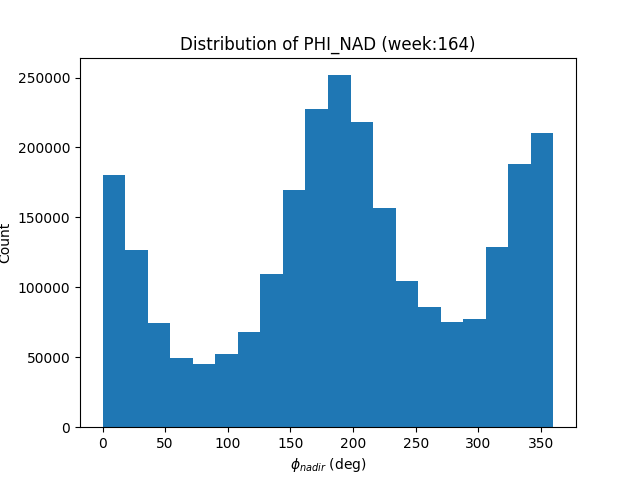
\includegraphics[width=0.47\textwidth]{content/result_and_discussion/figures/phi_nad_dist.png}
        }
        \caption{An example distribution of $\gamma$-ray from a single week.}
       \label{fig:sample_photon_dist}
\end{figure}

The limb's region could be easily observed in the bright ring above 
a dashed line of 60\textdegree $\theta_\text{NADIR}$.
Figure \ref{fig:sample_photon_dist} also shows the brightness of 
the southern and northern hemispheres. Further investigating of the 
East-West effects could be illustrated by projecting the 2-D histogram 
into a 1-D histogram of the nadir angle as in Figure \ref{fig:sample_photon_dist}b.
Nevertheless, the explanation of the East-West is a rough description
and still incomplete because it does not take
the exposure into account yet.

% Applying criteria from the data selection such as event class,
% LAT's incident angle would affect the result from
% the histogram filling.


\begin{figure}[h!]
    \centering
    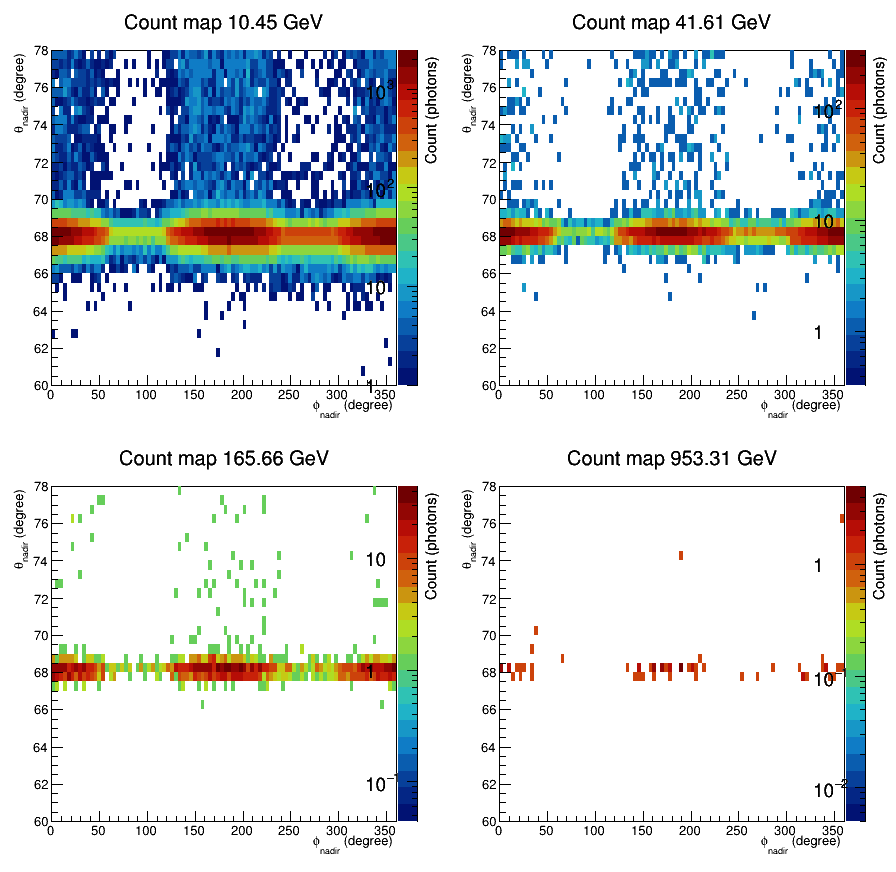
\includegraphics[width=0.8\textwidth]{content/result_and_discussion/figures/cartesian_cntmaps.png}
    \caption{
        Cartesian plot of the $\gamma$-ray count histograms.
        The title is each sub-figure represent
        mean of the energy bins.
    }
    \label{fig:cntmap_cartesian}
\end{figure}

Since the final spectrum will contain 50 energy bins
with their specific energy range and mean energy
for each energy bin.
In practice, each heatmap will be constructed
for their belonging bin of the histogram in the energy domain
as in the Figure \ref{fig:cntmap_cartesian}.


However, inspecting at polar coordinate plotting
from the cartesian point of view might not be the best option for 
illustration since it not looks like the real orientations.
Figure \ref{fig:cntmap_polar} is another
angle of viewing the same data but in more natural orientations.
Both visualizations show that the Earth's limb region in $\gamma$-ray 
is the shinest band for all interesting energy.
It is also obvious to say that the higher energy scale,
the less photon appears after applying criteria.


\begin{figure}[h!]
    \centering
    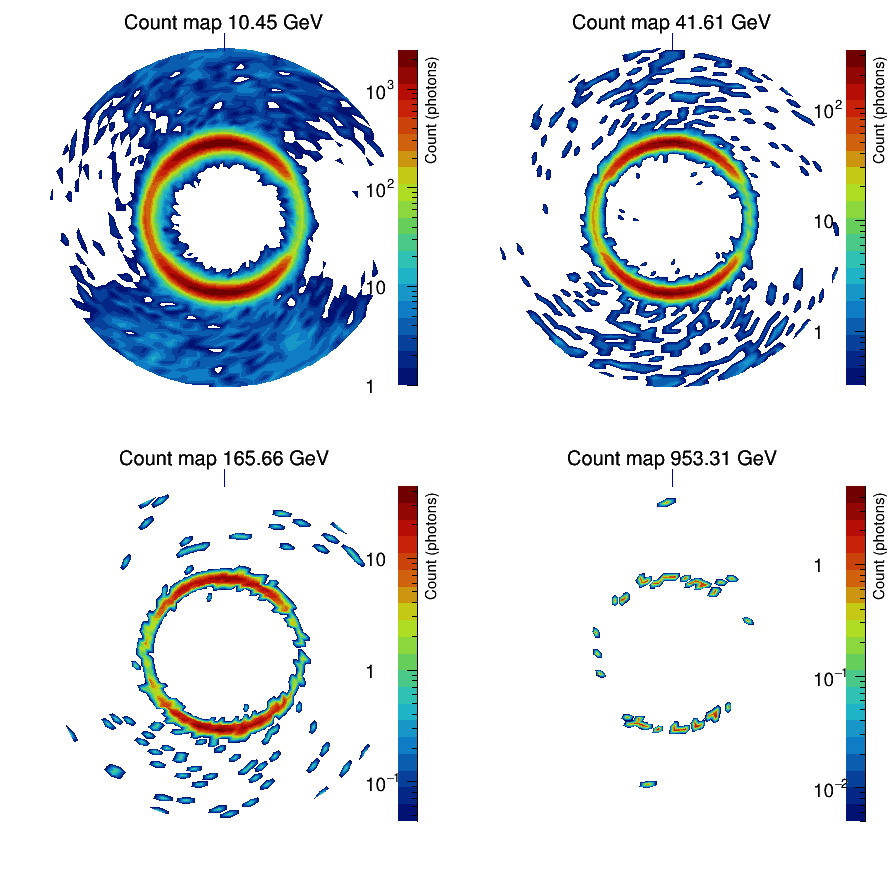
\includegraphics[width=0.8\textwidth]{content/result_and_discussion/figures/polar_cntmaps.png}
    \caption{Polar plot of the $\gamma$-ray count histograms.}
    \label{fig:cntmap_polar}
\end{figure}


The next step is the exposure calculation.
The exposure map is computed 
by accumulating exposure time from the LAT's FoV
in each step time as well as takes the 
effectiveness of the detector due to incident angle
affects the performance of the detector.
A unit from the calculation will be an 
area multiple by the time. Raw cartesian plots are visualized in
Figure \ref{fig:expmap_cartesian} with an attached axis.

\begin{figure}[h!]
    \centering
    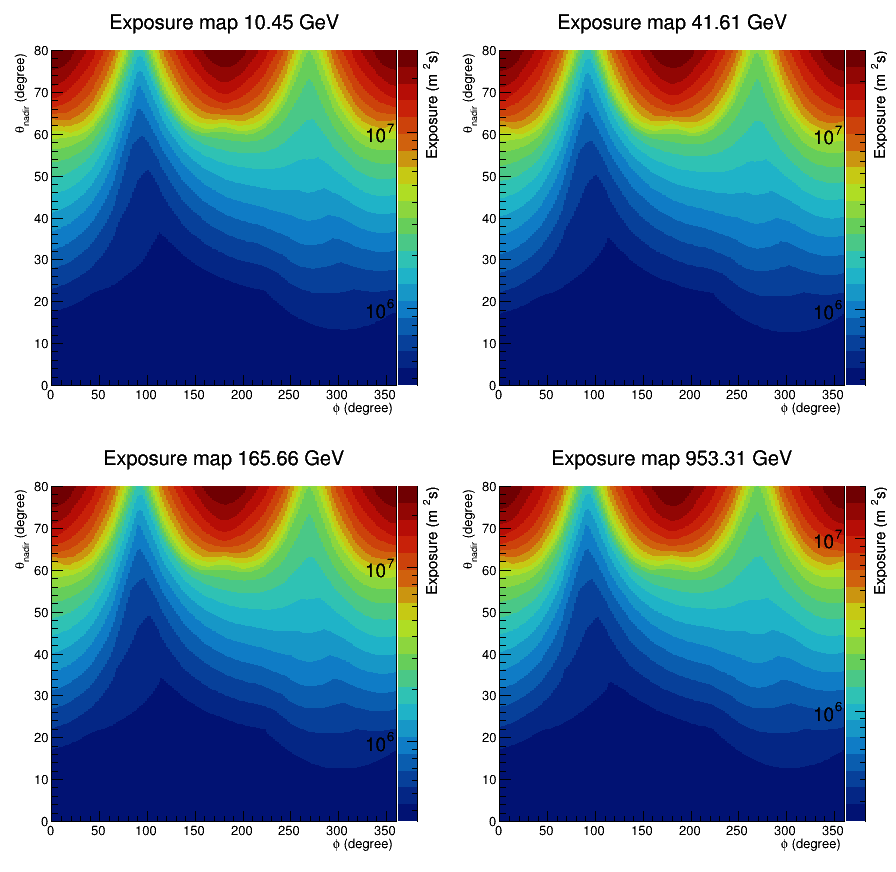
\includegraphics[width=0.8\textwidth]{content/result_and_discussion/figures/cartesian_expmaps.png}
    \caption{Cartesian plot of the exposure histograms.}
    \label{fig:expmap_cartesian}
\end{figure}


The exposure intensity in the sky is much
higher than the Earth in an order of magnitude
because \textit{Fermi} was designed
for seeking flare events in space rather than the Earth.
Regarding a given nadir angle between
60\textdegree to 70 \textdegree,
the spacecraft seems to look at the northern and southern hemisphere 
more than the eastern and the western side. The color of the 
at 270\textdegree (West) is more intense than 90\textdegree (East)
means that the spacecraft tends to peek in the Westside more
than Eastside. The reason might come from the
trajectory of the charged particles was bent
and produce a $\gamma$-ray which potentially could 
convince \textit{Fermi} to look at them rather
than the other side because it 
has a more for triggering the GBM.
The 2-D histograms in polar coordinates have also been
plotted in Figure \ref{fig:expmap_polar}.

\begin{figure}[h!]
    \centering
    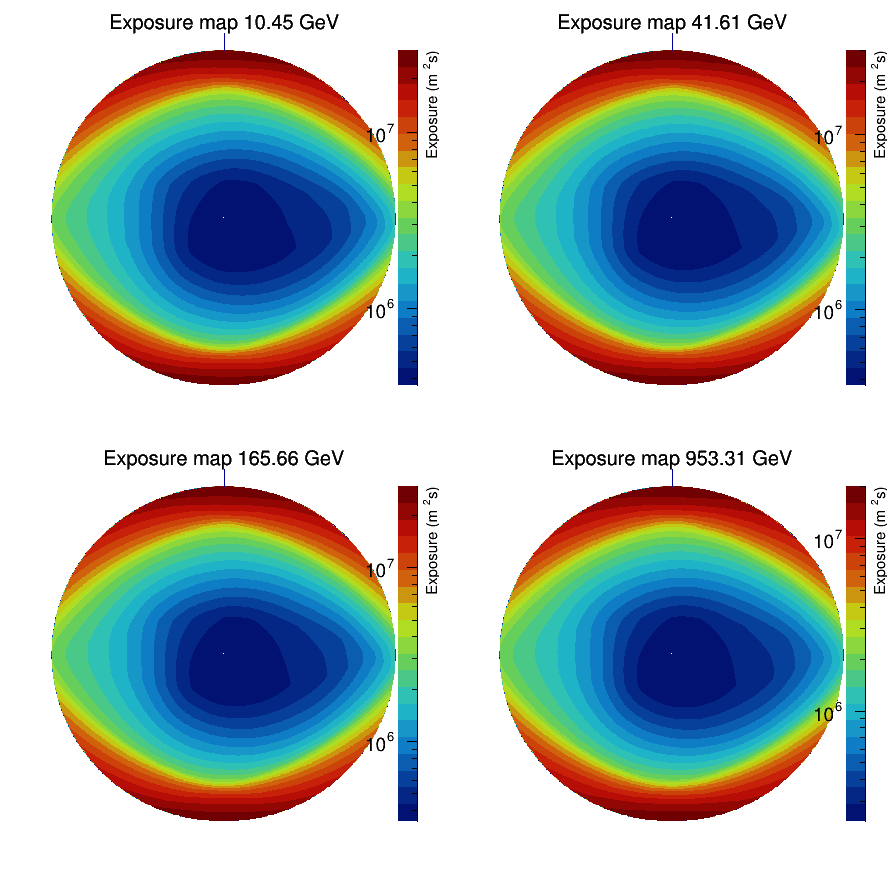
\includegraphics[width=0.8\textwidth]{content/result_and_discussion/figures/polar_expmaps.png}
    \caption{Polar plot of the exposure histograms.}
    \label{fig:expmap_polar}
\end{figure}


The last step starts with initiating the new heatmaps that were 
defined by the element-wise division from the
count maps and the exposure maps.
After that, integrating the limb region in the polar coordinates
to get a single scalar value. The scalar is then divided by the 
gap of the energy bin and the solid angle.
Repeating the above process for 50 energy bins in the $\gamma$-ray 
spectrum and subtracts by the background would yield the final 
photon spectrum as in Figure \ref{fig:flxhist}.

\begin{figure}[h!]
    \centering
    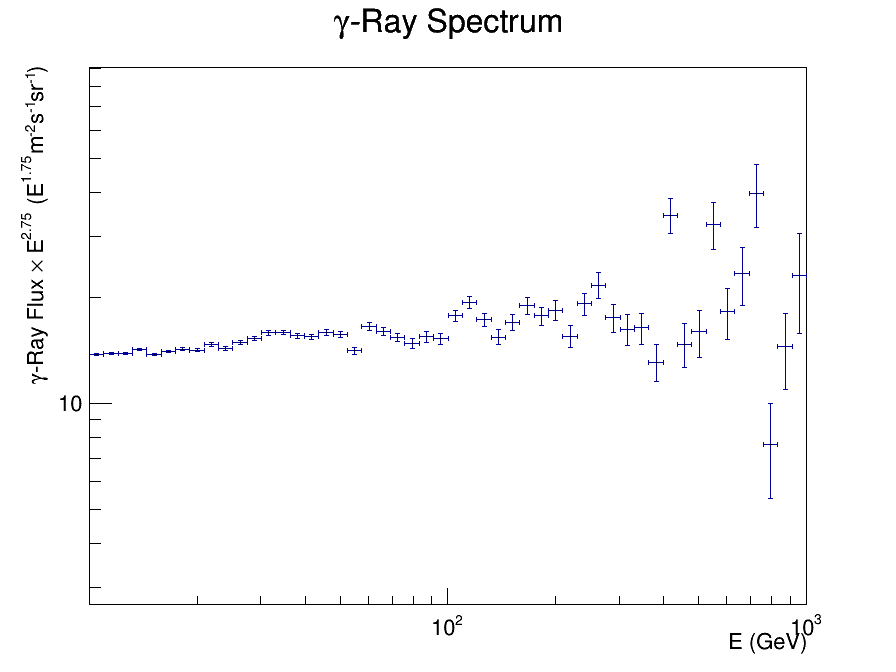
\includegraphics[width=0.7\textwidth]{content/result_and_discussion/figures/flx_hist.png}
    \caption{Measured $\gamma$-ray spectrum.}
    \label{fig:flxhist}
\end{figure}

In addition, exploring the $\gamma$-ray
intensity from the visualization
of the Earth's centered coordinates would be informative aspects
to observe the variation of the photon
intensity along the nadir angle as well as the 
East-West effect. The cartesian plotted is in Figure
\ref{fig:flxmap_cartesian} and the polar form as in the Figure 
\ref{fig:flxmap_polar}. Comparing the intensity along the peak of 
theta nadir in the cartesian plot from the East ($\phi$=90\textdegree)
and West ($\phi$=270\textdegree) would reflect that the band of 
the intensity in the west is slightly
thicker than in the East and the 
color of the peak center is more a little darker than the other 
side. It means that not only the intensity
but also the ring thickness
of the limb region is larger from West to East.


\begin{figure}[h!]
    \centering
    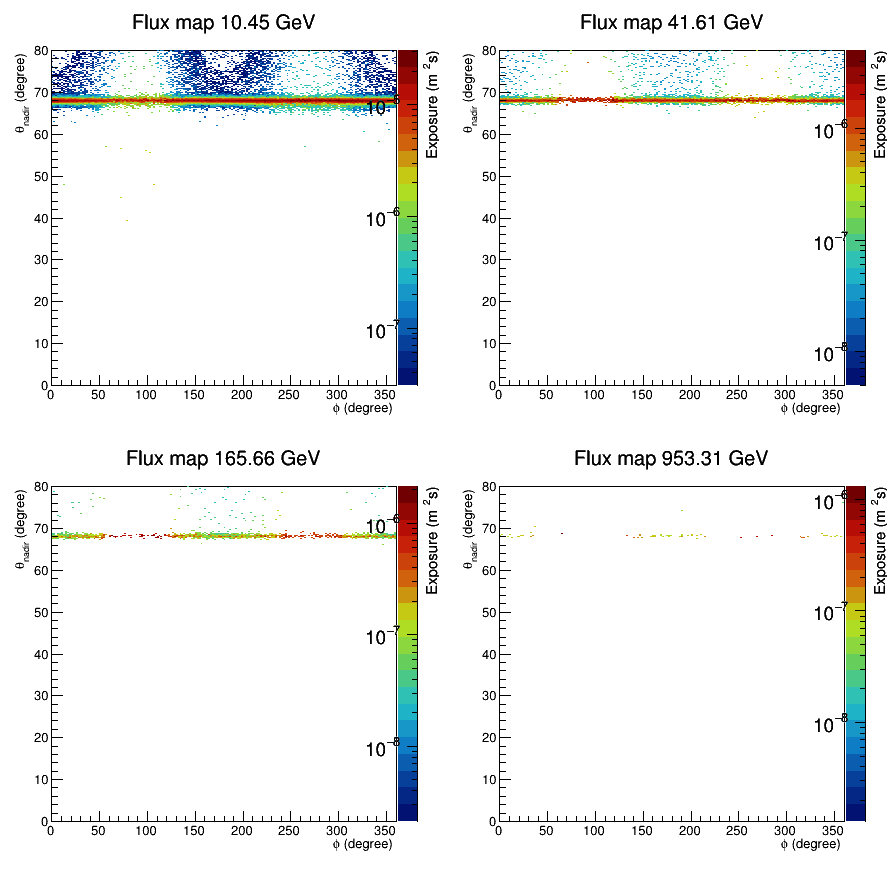
\includegraphics[width=0.8\textwidth]{content/result_and_discussion/figures/cartesian_flxmaps.png}
    \caption{Cartesian plot of the $\gamma$-ray flux histograms.}
    \label{fig:flxmap_cartesian}
\end{figure}


\begin{figure}[h!]
    \centering
    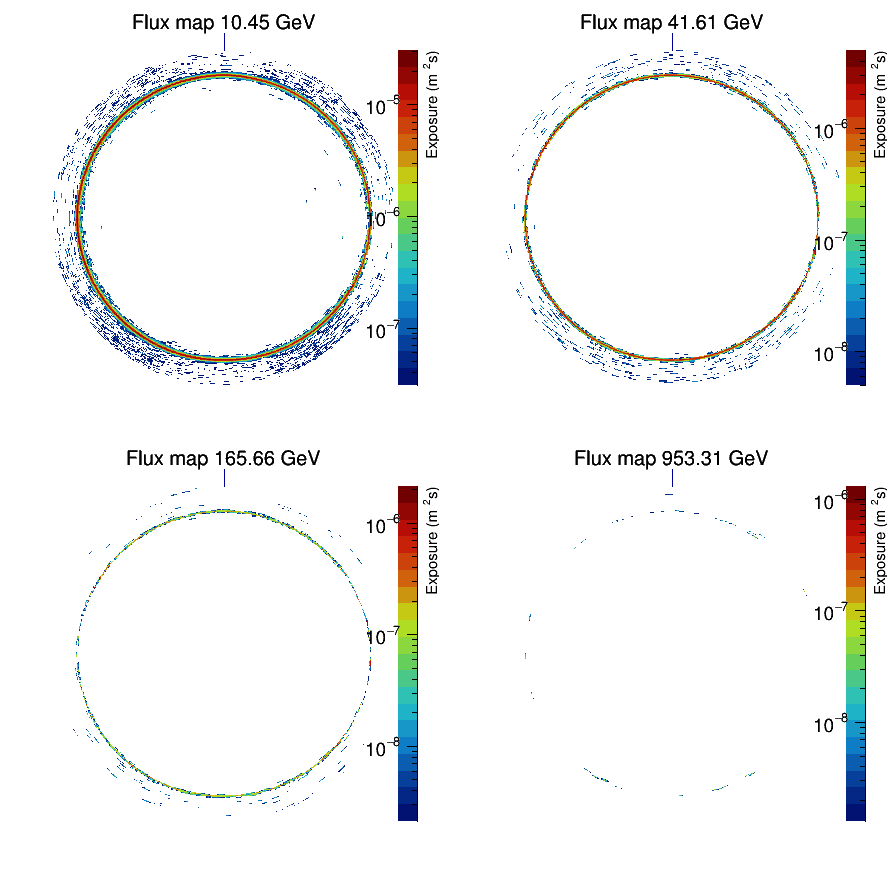
\includegraphics[width=0.8\textwidth]{content/result_and_discussion/figures/polar_flxmaps.png}
    \caption{Polar plot of the $\gamma$-ray flux histograms.}
    \label{fig:flxmap_polar}
\end{figure}

\newpage

\section{Best fit result}

The optimized parameters for SPL and BPL models are summarized in 
Table \ref{tb:bestfit}. Best fit $\gamma$-ray from both models are 
visualized in the Figure \ref{fig:fitted_gamma_specgtrum} along
with spectrum from the measurement. The result shows the consistency
between the direct measurement from AMS-02 and
the previous work. Both studies identify the breaking point 
of the spectral index in proton spectrum at $\sim$ 300 GeV as well 
as the previous work reported $\Gamma_1 \sim 2.81$
and $\Gamma_2 \sim 2.68$ for the BPL model.

\begin{table}[h!]
    \centering
    \begin{tabular}{l | c | c | c}
      Best fits & $\Gamma_1$ & $\Gamma_2$ & $E_{\text{Break}}$ (GeV) \\
      \hline \hline
      SPL & 2.70 & - & -  \\
      BPL & 2.86  & 2.63 & 333
    \end{tabular}
    \caption{Optimization results.}
    \label{tb:bestfit}
\end{table}

The comparative illustration
also be visualized in the Figure \ref{fig:fitted_cr_proton} with a 
scaled spectra from both models to collate two other direct 
observations of the space-based experiments. It is obvious to see 
the consistency of BPL with the direct measurements in the bellowing 
sub-figure is more corresponding than the SPL model in the top sub-figure
because the breaking point of the BPL does looks more likely to be 
a proper model where the x-axis is the same rigidity scale.

However, a more complex model would perform better than the model 
that has less degree of freedom in practice. Determining the 
statistical significance would be the best way to answer whether 
CR spectrum is naturally described as a BPL indeed.
The significant level could be determined by
taking the outcome from the objective function
to Equation \ref{eq:lrt} for testing one-tail hypothesis-like
from the null hypothesis comparing to an alternative
hypothesis which is the model of breaking of spectral indices
, or SPL versus BPL in other words.
The significance is around 1.38$\sigma$ or
at 92\% confidence level.


\begin{figure}[h!]
    \centering
    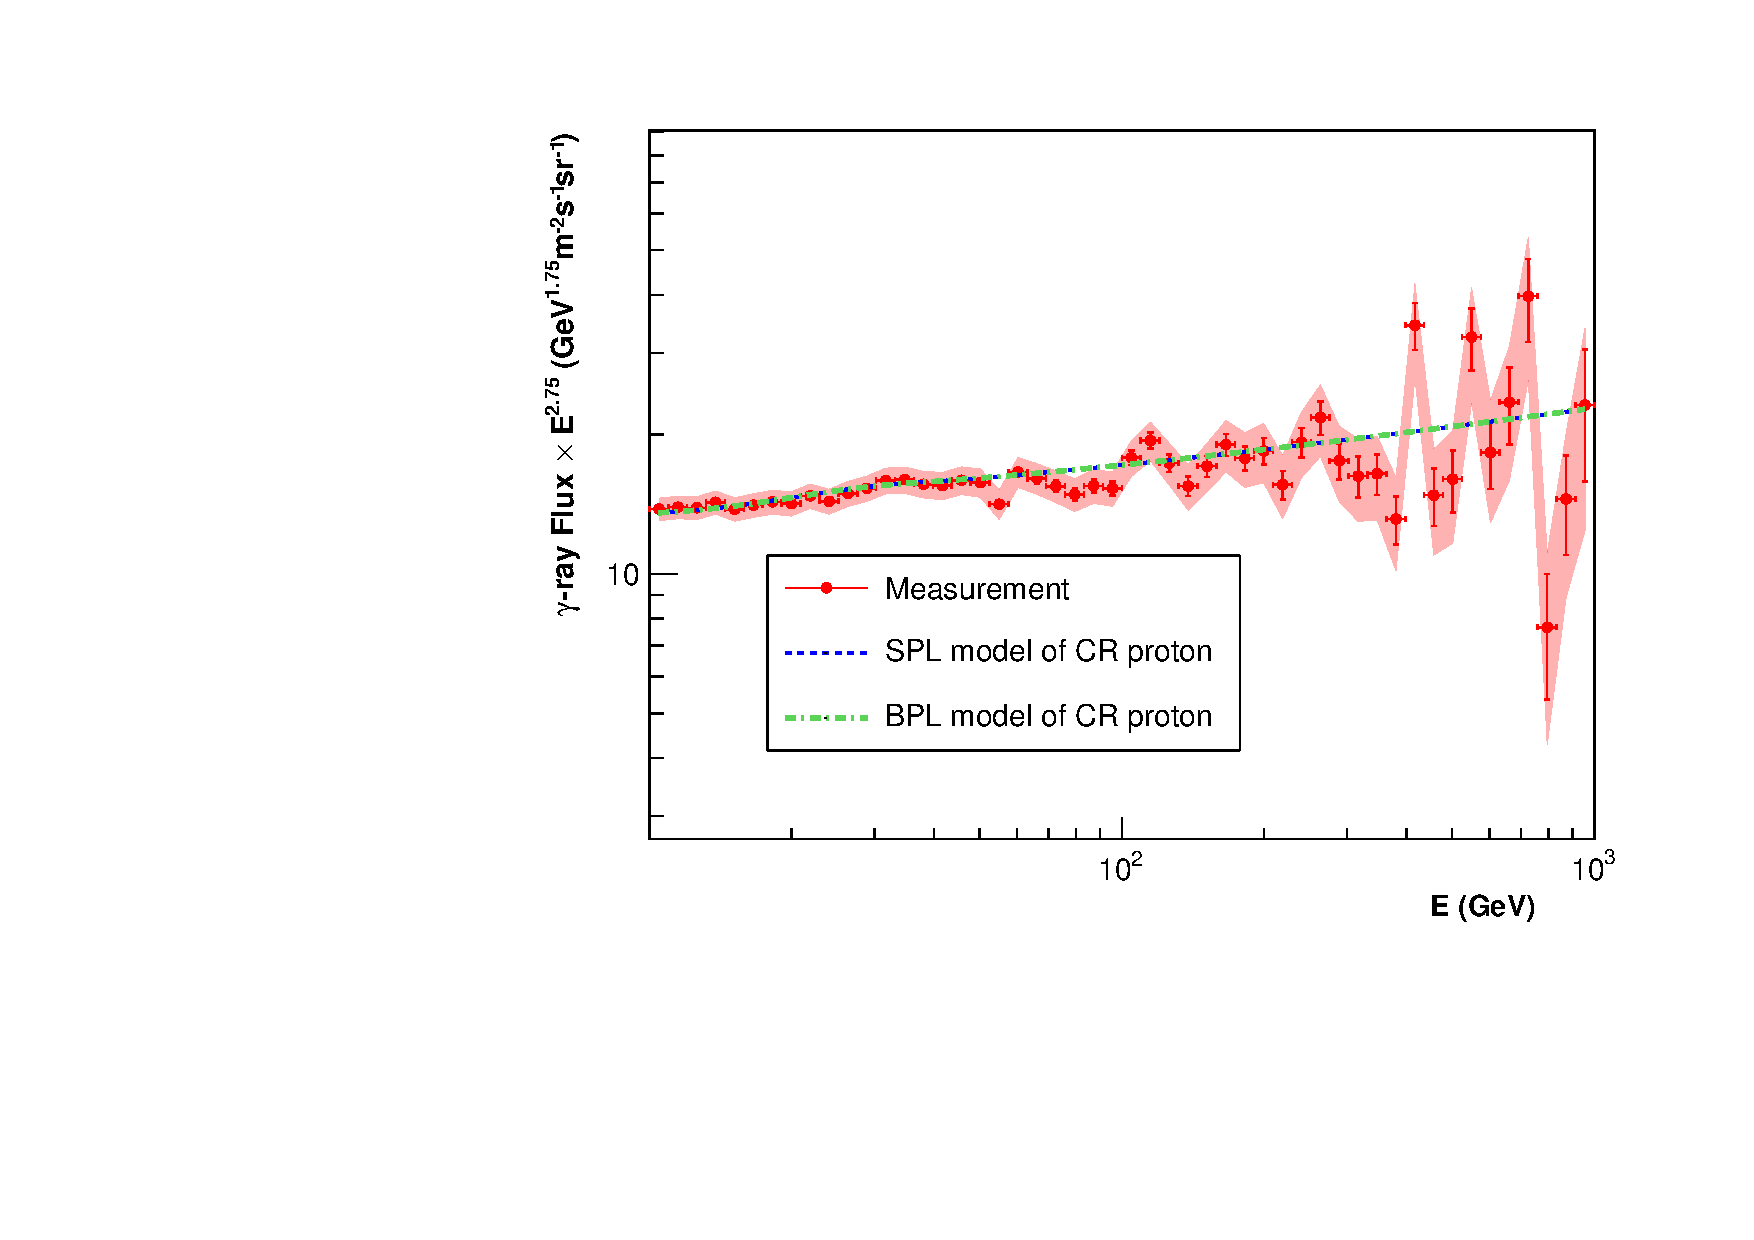
\includegraphics[width=0.8\textwidth]{content/result_and_discussion/figures/fitted_result.pdf}
    \caption{
        The $\gamma$-ray spectra calculated from the SPL (red)
        and BPL (blue) models of CR proton which best fit with the
        measured Earth's $\gamma$-ray spectrum in the thin-target
        regime (red).
    }
    \label{fig:fitted_gamma_specgtrum}
\end{figure}

\newpage 

\begin{figure}[h!]
    \centering
    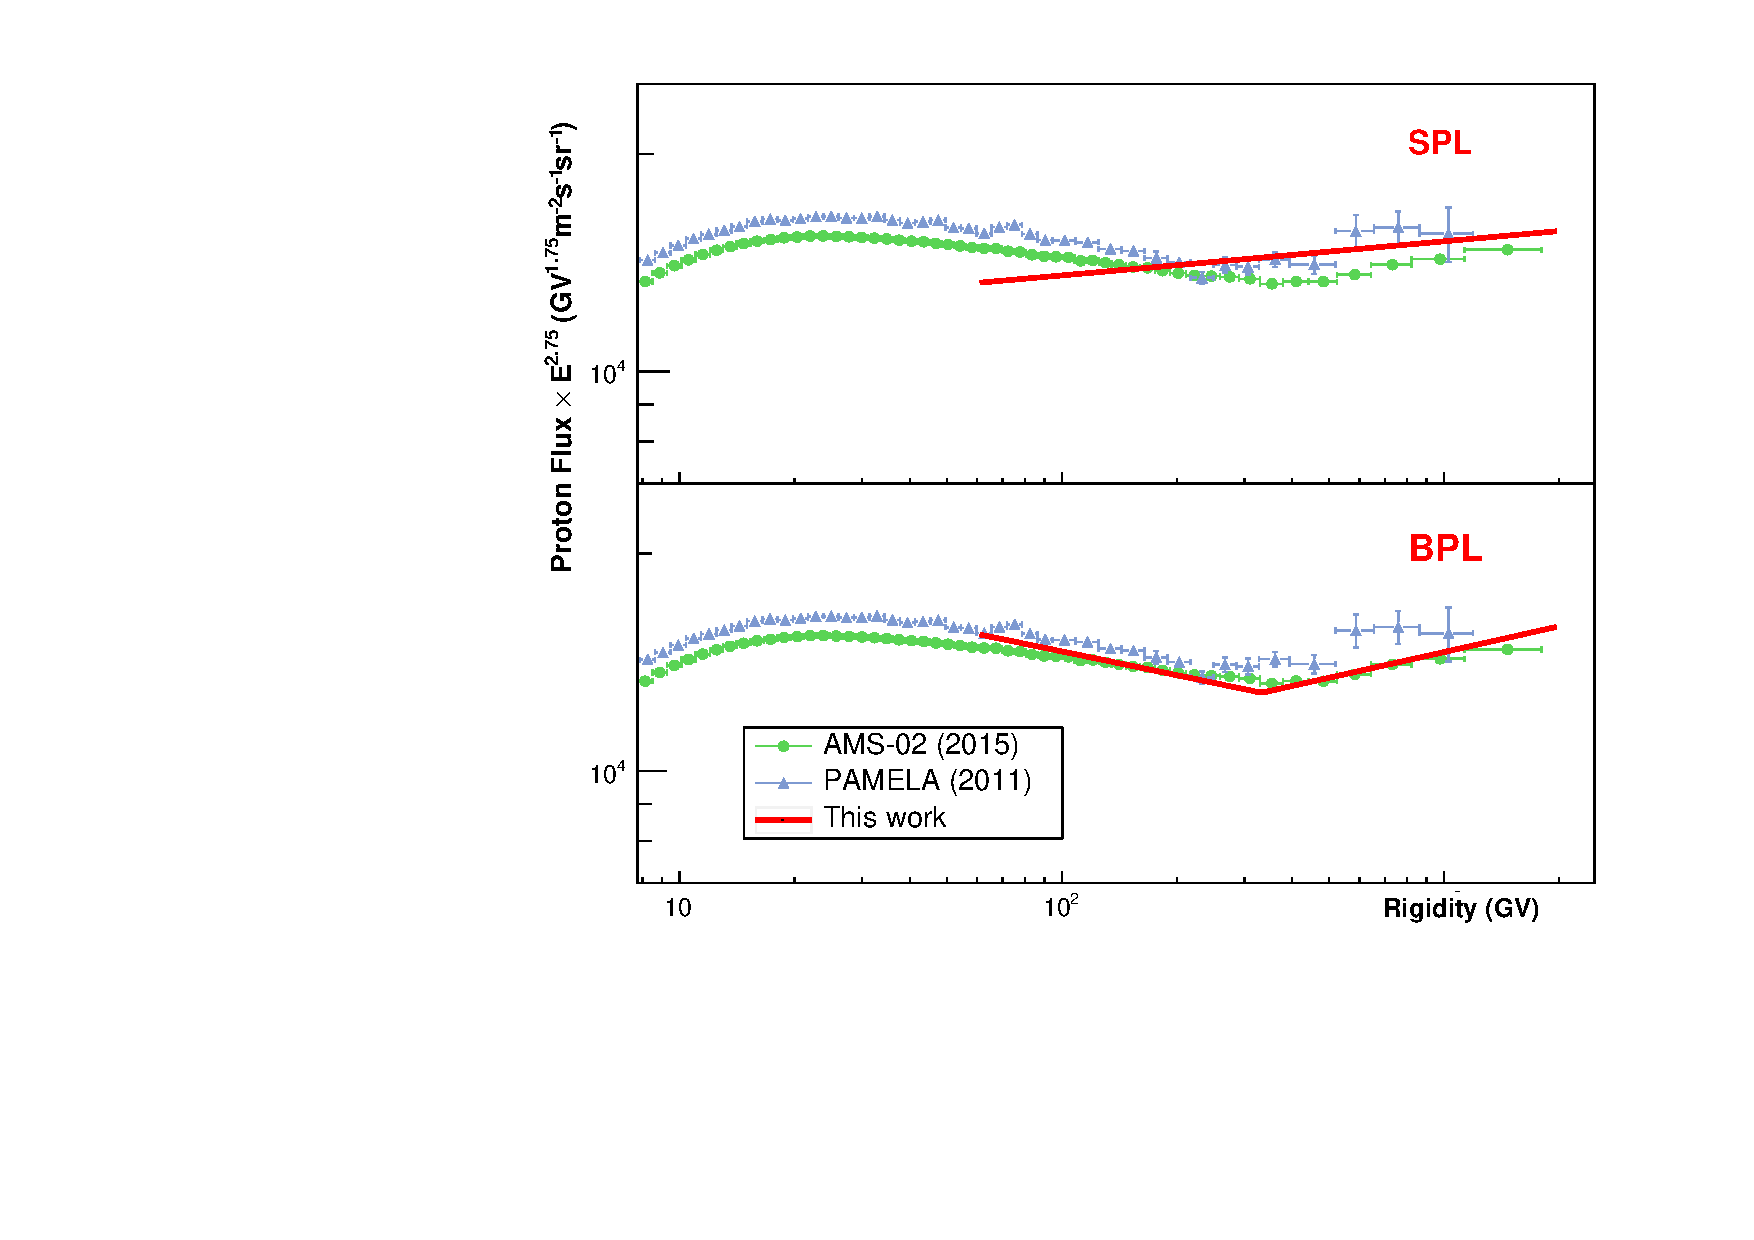
\includegraphics[width=0.9\textwidth]{content/result_and_discussion/figures/ProtonSpectrumModelMeasurement.pdf}
    \caption{
        Best-fit CR proton spectrum from this work (red)
        compared to the measurementsby AMS-02 (blue) and
        PAMELA (green).
    }
    \label{fig:fitted_cr_proton}
\end{figure}

